\documentclass[10pt]{report}
\usepackage[left=2cm, right=2cm, top=2cm]{geometry}
\usepackage{graphicx}

\begin{document}	
{\huge\hspace{210pt}R\'{e}sum\'{e}}
\\{\noindent\rule{18cm}{0.8pt}\\[4pt]}
\bf Address: \hspace{259pt}\bf Name:\verb| Bhaskar Dutt|
\\
\verb"H-69c,Mansarovar Park,"  \hspace{188pt}\bf Phone No:\verb" 7042513094"
\\{\verb"Shahdara,Delhi,"}   \hspace{225pt}\bf Email Id:\verb" bhaskarofficial2@gmail.com"
\\{\verb"110032"}    \hspace{272pt}\bf College:\verb" ADGITM(IPU DELHI)"
\\\hspace{250pt}\bf Github Link:\\\verb|https://github.com/bhaskarsdose| \\[1pt]
	                  

{\hspace{330pt}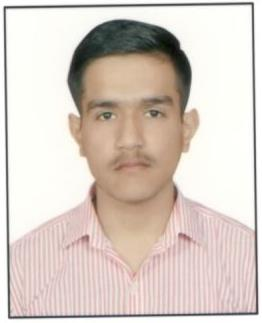
\includegraphics[scale =0.5]{bhaskar}\\[3pt]} % My image 
\section*{Objective:} % Details about my objective
\normalfont I am a tech enthusiast and a problem solver guy, I always believe that perseverance beat talent, therefore, I always try, I wanted to build or create new technologies which can help the masses or my country. As I am always interested in the defence sector my aim is to make India reliant on its own defence equipment production and always wanted to mimic the life of Dr.APJ Abdul Kalam sir.

\section*{Education:} % It houses my academic performance
\begin{center}
\begin{tabular}{|c|c|c|c|c|c|}
	\hline
	\hspace{2pt}\large\textbf{Degree} \hspace{2pt} & \hspace{2pt}\large\textbf{College/School}\hspace{2pt} &\hspace{2pt} \large\textbf{University}\hspace{2pt} &\hspace{2pt}\large\textbf{Passing Year}\hspace{2pt} & \hspace{2pt}\large\textbf{Passing Percentage/CGPA}\hspace{2pt}\\
	\hline
%	\multirow
	 B.Tech in EEE & ADGITM & I.P University Delhi & 2016-2020 & 8.4 \\
	XII & K.V.N.F.C & Kendriya vidyalaya & 2004-2016 & 89\%\\
	X & K.V.N.F.C & Kendriya vidyalaya & 2004-2014 & 8.8\\ 
	\hline
\end{tabular}
\end{center}

\section*{Projects:}%projects has been added and updated
 
\textbf{\large 1. Real-Time pollution monitor for air quality measurements\\[1pt] }
\\In this project I utilized the raspberry pi 3b+ as a local server to host a webpage as well as to connect various nodes through mosquitto channel on the other hand I have used nodemcu to interface with sensors like bme680,sharp dust sensor and mq135 to measure the data like temprature,pressure,humidity,AQI,NO2,SO2,CO2, PM10\&2.5 and send it to the server to log the data as well as for live display.
\\\textbf{Video link:-} https://youtu.be/qMB781NHcqE
\\\textbf{Project link:-} https://github.com/bhaskarsdose/Air-Monitoring-System \\               https://github.com/bhaskarsdose/AWS-based-Air-quality-logger-/\\[2pt]
	 
\noindent\textbf{\large 2. Smart energy logger and meter\\[1pt]}
\\I am working in building a device which measures multiple parameters like current,voltage,frequency and temperature for various purposes like energy monitoring, battery health and to make some real-time observation of what is electricity consumption for the purpose of increasing efficiency and health of the whole systems like in factories there is lot of energy wasted due to nonavailability of smart measuring devices which collects the data by the help of which we can improve a lot of things.
\\\textbf{Project Link:-} https://github.com/bhaskarsdose/SMART\_ENERGY\_METER\\[2pt]

\noindent\textbf{\large 3. Real-time heart rate and temperature monitor using IoT\\[1pt]}
\\This project is been selected at vihaan 2.0 hackathon of dtu Delhi In this project we used thingspeak API and created an app through MIT app inventor, On which we get the live data of heart rate and temperature sensor,After this the data go into the Thingspeak API where we used simple algorithms to build the graphs/plots and our next motive is to compare this data by prebuilt dataset which can help the patient in real life.
\\\textbf{Project Link:-} https://github.com/bhaskarsdose/micro-health-monitoring-system\\[2pt]

\noindent\textbf{\large 4. Geyser feedback circuit\\[1pt]}
\\In this project, we used thyristor(negative coefficient one) to sense the temperature by the help of which the feedback circuit gets its input which in turn with the help of npn transistors turn ON and OFF the relay connected with it which finally cut off and on the main supply to the heating aliment,this project is simply a basic prototype for understanding the working of various electronic components and their switching.\\[2pt]

\noindent\textbf{\large 5. Smart Socket\\[1pt]}
\\This my internship project or mine first IoT based project from which I learnt PCB designing, relay control circuit, nodemcu interfacing and connecting it to the internet or locally using bluetooth hc-05 to give its command for turning on and off the appliances connected with the socket , Along with that I also integrated this with the \textbf{IFTTT} template to turn on and off the relay using the google voice assistent as it generates the instance which goes to the cloud which send the command to the applet.
\\\textbf{Project Link:-} https://github.com/bhaskarsdose/IOT-enabled-socket\\[2pt]

\noindent\textbf{\large 6. Smart water monitoring and management system\\[1pt]}
\\This project basically work as an automatic control system for the water pumps in this we used two nodemcu which communicate with each other to turn ON and OFF the motor , one nodemcu is connected at the water tank with ultrasonic sensor which measures the water level and other with the relay to disconnect or connect the supply with the motor.\\[2pt] 

\noindent\textbf{\large 7. Mini quadcopter\\[1pt]}
\\I am currently working on this project using eachine flight controller using this we can do a certain task easily which we can define later.
\\\textbf{Link:-} https://drive.google.com/file/d/1tPTBw8y6eKShXya8BZ4sjXn9a4iqKP7c/view?usp=drivesdk




\section*{Trainings \&\\ Internships:} % section for my internships
\begin{itemize}
\item Done training on plc and scada.
\item Intern at W3Dev (a startup by IIITD student) as an IOT(Internet of things) Developer for 2 months from June 2018 to August 2018.
\item working as hardware developer (iot) in algo8 under the name of power8 for the last 4 months.
\end{itemize}

\section*{Research \\Publications:} %Details about research publications
\begin{enumerate}
	\item Written research paper on \textbf{\textit{"Automation in factories using Internet of Things(IoT)"}} published in the IETET journal   PAPER ID \#A17.
\end{enumerate}


\section*{Technical \\Skills:} %my technical skills AF :))))))
\begin{itemize}
\item Have relevant knowledge of INDUSTRIAL AUTOMATION like controllers for DG's.
\item Languages knew C++,Python,C.
\item PCB Designing.
\item Internet Of Things(IoT) --- "MAJOR SKILL". 
\item Have good experience in EMBEDDED SYSTEM Design.
\item Microcontroller used - ARDUINO, NODEMCU ESP-12e, EACHINE FC, ESP8266.
\item socket programming and API integration for IoT applications like for real world deployment.
\item Cloud computing.
\item Cloud used - thingspeak,google firebase,aws(dynamoDB) etc.
\item Hardware system developer.
\item worked on Augmented reality using openCV and openGL.
\item Microprocessor used - Raspberry pi 3b+ and pi zero.
\item worked on plc and scada.
\item Technical writing.
\item Blender objects designing.
\end{itemize}

\section*{Soft \\Skills:} % soft skills are here :)))))
\begin{enumerate}
	\item Workaholic,always try to complete the work given ASAP.
	\item Ability to accept failures as I know there are no failures only learning.
	\item Good time management.
	\item Team management skills.
	\item leadership capability.
	\item Public speaking.
	\item Good communication skills.
\end{enumerate}

\section*{Extra-\\Curricular\\Activities:} %extra curricular activites are here :))))
\begin{itemize}
	\item Blogging. check out my blog at bhaskarsdose.wordpress.com
	\item Teacher for many students as I teach maths to high school students and help juniors of my college in various projects.
	\item A prominent reader like I read daily newspaper and love to read biographies of great personalities like Dr.APJ Abdul Kalam ji, Bhagat Singh ji, Elon musk and jack ma etc.
	\item An avid debater on the topic of politics, history and ethics.
\end{itemize}

\section*{Co-\\Curricular\\Activities:}%extra curricular activities are here :)))))
\begin{enumerate}
	\item One of the organizer of T-HACK, official hackathon of IEEE NIEC.
	\item Membership coordinator at IEEE NIEC.
	\item Ex-project coordinator at our college IEEE branch. 
	\item Team leader for various hackathon conducted across different colleges like vihaan 2.0 dtu,IIIT Delhi hackathon and arduino day hackathon etc.
	\item Team leader for the team which selected for e yantra robotics competition 2018 finals at IIT Bombay.
	\item Been to SSB 4 times.
\end{enumerate}

\section*{Personal Details:}% details for cooman use are there like names
\textbf{Father's Name:} Mr.Narayan Dutt Sharma\\
\textbf{Mother's Name:} Mrs.Sheela Sharma\\
\textbf{Sex:} Male\\
\textbf{Date Of Birth:} 16 January 1999\\
\textbf{Nationality:} Indian\\
\textbf{Marital Status:} Single



\end{document}